%--------------------------------------------------------
\documentclass[10pt]{jarticle}
%----------------------------------------
%パッケージ
%----------------------------------------
\usepackage[top=20truemm,bottom=20truemm,left=20truemm,right=20truemm]{geometry}
\usepackage{amsmath,amssymb}
\usepackage{eucal}
\usepackage{bm}
\usepackage{ascmac}
\usepackage{pifont}
\usepackage{multirow}
\usepackage{enumerate}
\usepackage{cases}
\usepackage{url}
\usepackage[caption=false]{subfig}
\usepackage[ruled,vlined]{algorithm2e}
\usepackage{setspace}
\DeclareRelationFont{JY1}{mc}{it}{}{OT1}{cmr}{it}{}
\DeclareRelationFont{JT1}{mc}{it}{}{OT1}{cmr}{it}{}
\DeclareFontShape{JY1}{mc}{m}{it}{<5> <6> <7> <8> <9> <10> sgen*min
    <10.95><12><14.4><17.28><20.74><24.88> min10
    <-> min10}{}
\DeclareFontShape{JT1}{mc}{m}{it}{<5> <6> <7> <8> <9> <10> sgen*tmin
    <10.95><12><14.4><17.28><20.74><24.88> tmin10
    <-> tmin10}{}
\DeclareRelationFont{JY1}{mc}{sl}{}{OT1}{cmr}{sl}{}
\DeclareRelationFont{JT1}{mc}{sl}{}{OT1}{cmr}{sl}{}
\DeclareFontShape{JY1}{mc}{m}{sl}{<5> <6> <7> <8> <9> <10> sgen*min
    <10.95><12><14.4><17.28><20.74><24.88> min10
    <-> min10}{}
\DeclareFontShape{JT1}{mc}{m}{sl}{<5> <6> <7> <8> <9> <10> sgen*tmin
    <10.95><12><14.4><17.28><20.74><24.88> tmin10
    <-> tmin10}{}
\DeclareRelationFont{JY1}{mc}{sc}{}{OT1}{cmr}{sc}{}
\DeclareRelationFont{JT1}{mc}{sc}{}{OT1}{cmr}{sc}{}
\DeclareFontShape{JY1}{mc}{m}{sc}{<5> <6> <7> <8> <9> <10> sgen*min
    <10.95><12><14.4><17.28><20.74><24.88> min10
    <-> min10}{}
\DeclareFontShape{JT1}{mc}{m}{sc}{<5> <6> <7> <8> <9> <10> sgen*tmin
    <10.95><12><14.4><17.28><20.74><24.88> tmin10
    <-> tmin10}{}
\DeclareRelationFont{JY1}{gt}{it}{}{OT1}{cmbx}{it}{}
\DeclareRelationFont{JT1}{gt}{it}{}{OT1}{cmbx}{it}{}
\DeclareFontShape{JY1}{mc}{bx}{it}{<5> <6> <7> <8> <9> <10> sgen*goth
    <10.95><12><14.4><17.28><20.74><24.88> goth10
    <-> goth10}{}
\DeclareFontShape{JT1}{mc}{bx}{it}{<5> <6> <7> <8> <9> <10> sgen*tgoth
    <10.95><12><14.4><17.28><20.74><24.88> tgoth10
    <-> tgoth10}{}
\DeclareRelationFont{JY1}{gt}{sl}{}{OT1}{cmbx}{sl}{}
\DeclareRelationFont{JT1}{gt}{sl}{}{OT1}{cmbx}{sl}{}
\DeclareFontShape{JY1}{mc}{bx}{sl}{<5> <6> <7> <8> <9> <10> sgen*goth
    <10.95><12><14.4><17.28><20.74><24.88> goth10
    <-> goth10}{}
\DeclareFontShape{JT1}{mc}{bx}{sl}{<5> <6> <7> <8> <9> <10> sgen*tgoth
    <10.95><12><14.4><17.28><20.74><24.88> tgoth10
    <-> tgoth10}{}
\DeclareRelationFont{JY1}{gt}{sc}{}{OT1}{cmbx}{sc}{}
\DeclareRelationFont{JT1}{gt}{sc}{}{OT1}{cmbx}{sc}{}
\DeclareFontShape{JY1}{mc}{bx}{sc}{<5> <6> <7> <8> <9> <10> sgen*goth
    <10.95><12><14.4><17.28><20.74><24.88> goth10
    <-> goth10}{}
\DeclareFontShape{JT1}{mc}{bx}{sc}{<5> <6> <7> <8> <9> <10> sgen*tgoth
    <10.95><12><14.4><17.28><20.74><24.88> tgoth10
    <-> tgoth10}{}
\DeclareRelationFont{JY1}{gt}{it}{}{OT1}{cmr}{it}{}
\DeclareRelationFont{JT1}{gt}{it}{}{OT1}{cmr}{it}{}
\DeclareFontShape{JY1}{gt}{m}{it}{<5> <6> <7> <8> <9> <10> sgen*goth
    <10.95><12><14.4><17.28><20.74><24.88> goth10
    <-> goth10}{}
\DeclareFontShape{JT1}{gt}{m}{it}{<5> <6> <7> <8> <9> <10> sgen*tgoth
    <10.95><12><14.4><17.28><20.74><24.88> tgoth10
    <-> tgoth10}{}
\endinput
%%%% end of jdummy.def
\usepackage{here}
\usepackage[dvipdfmx]{graphicx}
\usepackage[dvipdfmx]{color}
%----------------------------------------
%各設定
%----------------------------------------
\setlength{\columnsep}{3zw}
\makeatletter
\newcommand{\figcaption}[1]{\def\@captype{figure}\caption{#1}}
\newcommand{\tblcaption}[1]{\def\@captype{table}\caption{#1}}
\renewcommand{\thefigure}{\arabic{figure}}
\@addtoreset{figure}{section}
\renewcommand{\thetable}{\arabic{table}}
\@addtoreset{table}{section}
\renewcommand{\theequation}{.\arabic{equation}}
\@addtoreset{equation}{section}
\makeatother
\renewcommand{\figurename}{Fig.}
\renewcommand{\tablename}{Table}

\renewcommand{\thesection}{12.\arabic{section}} % セクションの前に章番号を追加

%----------------------------------------

%----------------------------------------
\title{\vspace{-20truemm}
{\normalsize \rightline{2017 年\ 6月\ 26日}}  %日付
{\Large 知能システム学特論 第 2 回 レポート\\} %題目
\date{}
\vspace{-3truemm}}
%----------------------------------------
\author{
DL 4 班 \\
17344217 西尾 貴樹,
17344218 二宮 舜,
17344219 二宮 悠二,
17344226 山下 貴大
} %番号氏名
%--------------------------------------------------------
\begin{document}
\parindent = 0pt % 字下げOFF
\maketitle
%\thispagestyle{empty} % ページ番号 OFF
%--------------------------------------------------------
\vspace{-1.0cm}
\section{進捗状況}
%--------------------------------------------------------
\ \ 現在の進捗状況を以下に示す.
%-------------------------------
\begin{itemize}
\item 開発を行うテーマを決定した.
% \item DL によるグレイスケール画像のカラー復元に関する論文調査を行った.
\item 既存手法の課題を探し,改善策の検討を行った.
\item 提案手法に用いるアルゴリズムの検討を行なった.
\item いくつかデータセットを用意し,アルゴリズムの検証を行なった.
\end{itemize}
%-------------------------------
%--------------------------------------------------------
% \section{カラー復元に関する論文調査}
% %--------------------------------------------------------
% \ \ 飯塚ら(早稲田大学)の手法 \cite{waseda} について調査し,改善できる点がないか探した.
% %--------------------------------------------------------
\section{テーマの決定}
%--------------------------------------------------------
本講義において,私たちはモノクロ画像のカラー復元をニューラルネットワークを用いて構築する.これを実装するにあたり,先行研究としてある飯塚ら(早稲田大学)の手法 \cite{waseda} について調査し,改善できる点を探した.
%--------------------------------------------------------
\vspace{-0.4cm}
\subsection{手法の概要}
%--------------------------------------------------------
\ \ 提案されている手法では,ネットワークの前半部分に画像分類で用いられる畳み込みニューラルネットワークを配置し,大域的な特徴の抽出を行っている.そして,後半部分の層で局所的な特徴を抽出し,これらの特徴を併合した後,カラー復元を行っている.従来手法では色の指定に利用者の助けが必要であったが,提案手法ではデータセットを適切に用意すれば完全に自動で色を復元できる.また,人間にとって自然な色を復元するため,ニューラルネットワークの出力の色表現としては CIE L*a*b 色空間を利用している.入力画像の解像度に依らず,画質を維持した状態でのカラー復元が可能となっている.
%--------------------------------------------------------
\vspace{-0.2cm}
\subsection{改善策の提案}
%--------------------------------------------------------
\ \ 提案手法では望ましい出力とされるカラー画像が複雑な配色だった場合や,色の候補が複数で定まらない場合に,カラー復元の性能が落ちてしまうことがある.これは,全ての入力画像に対するカラー復元を一つのニューラルネットワークで行っているためだと考えられる.すなわち,学習に用いるデータセットが表現するデータ範疇を越えた入力に対応できていない.これを改善する方法として, {\bf Fig.~\ref{fig:cnn_class}} に示すような手法が考えられる.この手法では,入力画像を人物,風景,料理などのカテゴリに分類するニューラルネットワークと,それぞれのカテゴリの着色に特化したニューラルネットワークを構築する.全てのニューラルネットワークの学習が完了した後,グレースケール画像はカテゴリ分類器に入力される.その後,分類器の分類結果に該当するカテゴリについて,最適な着色を行うニューラルネットを選んでカラー復元を行う.ただし,この手法ではカラー復元を行うニューラルネットワークはカテゴリの数だけ必要となる.
%-------------------------------
\begin{figure}[tb]
\centering
  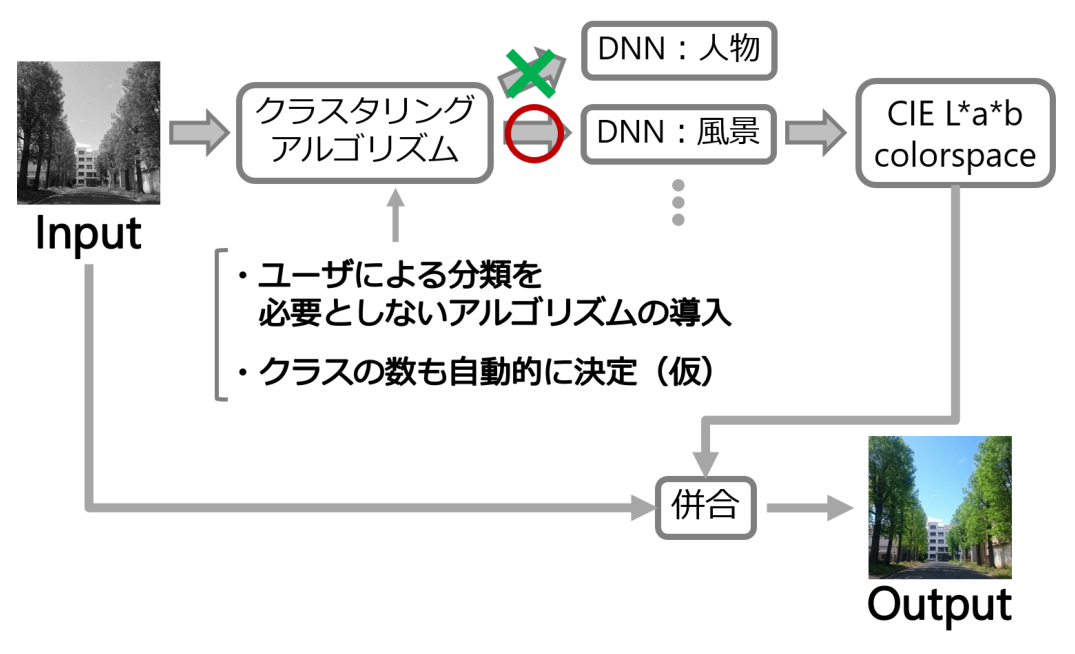
\includegraphics[scale=0.5]{../figures/flow.eps}
\caption{Colorization with CNN classification.}
\label{fig:cnn_class}
\end{figure}
%-------------------------------
\section{アルゴリズムの検討}
%--------------------------------------------------------
\subsection{画像分類}
%--------------------------------------------------------
\ \ 本提案手法にて用いる画像分類の代表的なアルゴリズムとして K-近傍法が挙げられる.画像の特徴量を検出しクラスを分類する.
一方,ニューラルネットワークを用いる場合,何を指標として扱うか,またクラスの数はどうするのかという問題が挙げられる.これらについては検討中である.
%--------------------------------------------------------
\subsection{着色を行うDNN}
%--------------------------------------------------------
\ \ 着色には DNN を用いる.畳み込み層によるダウンサンプリング,正規化層,逆畳み込み層によるアップサンプリングを経て CIE L*a*b 色情報を得る.こうして得られた色情報と入力のグレースケール画像を併合させ,カラー化を図る.
\section{ニッシーのゼミ一回分の功績}
%--------------------------------------------------------
\ \ 存分に語ってくれたまえよ.
%--------------------------------------------------------
\section{今後の予定}
%--------------------------------------------------------
\ \ クラス分類の箇所にどのような手法を取り入れるのか決定し,まずは少ないデータセット量から実際に分類ができるのか実行していく予定である.
%--------------------------------------------------------
\begin{thebibliography}{99}
\addcontentsline{toc}{section}{参考文献}
%-------------------------------
\bibitem{waseda} Iizuka Satoshi, Edgar Simo-Serra, and Hiroshi Ishikawa. ``Let there be color!: joint end-to-end learning of global and local image priors for automatic image colorization with simultaneous classification.'' ACM Transactions on Graphics (TOG) 35.4 (2016): 110.
%-------------------------------
\bibitem{style} Gatys Leon A., Alexander S. Ecker, and Matthias Bethge. ``Image style transfer using convolutional neural networks.'' Proceedings of the IEEE Conference on Computer Vision and Pattern Recognition. 2016.
%-------------------------------
\end{thebibliography}
\end{document}
